\documentclass[12pt]{article}
\usepackage{graphicx}
\usepackage{amsmath}
\usepackage{geometry}
\usepackage{tikz} % for drawing graphs
\usetikzlibrary{arrows.meta}
\usetikzlibrary{positioning}
\usepackage{listings} % for code listings

\geometry{margin=1in}

\lstset{
    backgroundcolor=\color{gray!10}, % Light grey background
    basicstyle=\ttfamily,             % Use a monospaced font
    frame=single,                     % Add a frame around the code
    rulecolor=\color{black},          % Frame color
    upquote=true,                      % Use straight quotes
	numbers=left,                     % Line numbers on the left
	numbersep=5pt,                    % Gap between line numbers and code
	numberstyle=\color{black},    % Line numbers are grey and small
	% Keywords
	keywordstyle=\color{blue},        % Keywords are blue
	% Comments
	commentstyle=\color{green},       % Comments are green
	% Strings
	stringstyle=\color{red},          % Strings are red
	breaklines=true,                  % Wrap long lines
	showstringspaces=false            % No special string spaces
}

\begin{document}

\title{Assignment 2: Implementing Sorting Algorithms in C and Creating a Shared Library for Python with Case Study}
\author{Talha Ahmad, 400517273}
\date{October 13, 2024}
\maketitle

\section{Introduction}

In this assignment, I implemented 4 sorting algorithms in C: Insertion, Merge, Heap, and Counting Sort.
The assignment file came with an implementation of the Bubble Sort algorithm, which I did not modify.
In this report, I will aim to discuss how each algorithm works, the time complexity of each algorithm, and the results of running the algorithms on a set of random integers.

\section{Sorting Algorithms}

\subsection{Bubble Sort}

Bubble Sort iterates through a list of elements and compares adjacent elements, swapping them if they are in the wrong order.
This process is repeated until the list is sorted.
Typically, this is implemented with two nested loops, where the outer loop iterates through the list and the inner loop iterates through the list - 1 elements checking and swapping adjacent elements.
The following graphic demonstrates the process of Bubble Sort:

\begin{center}
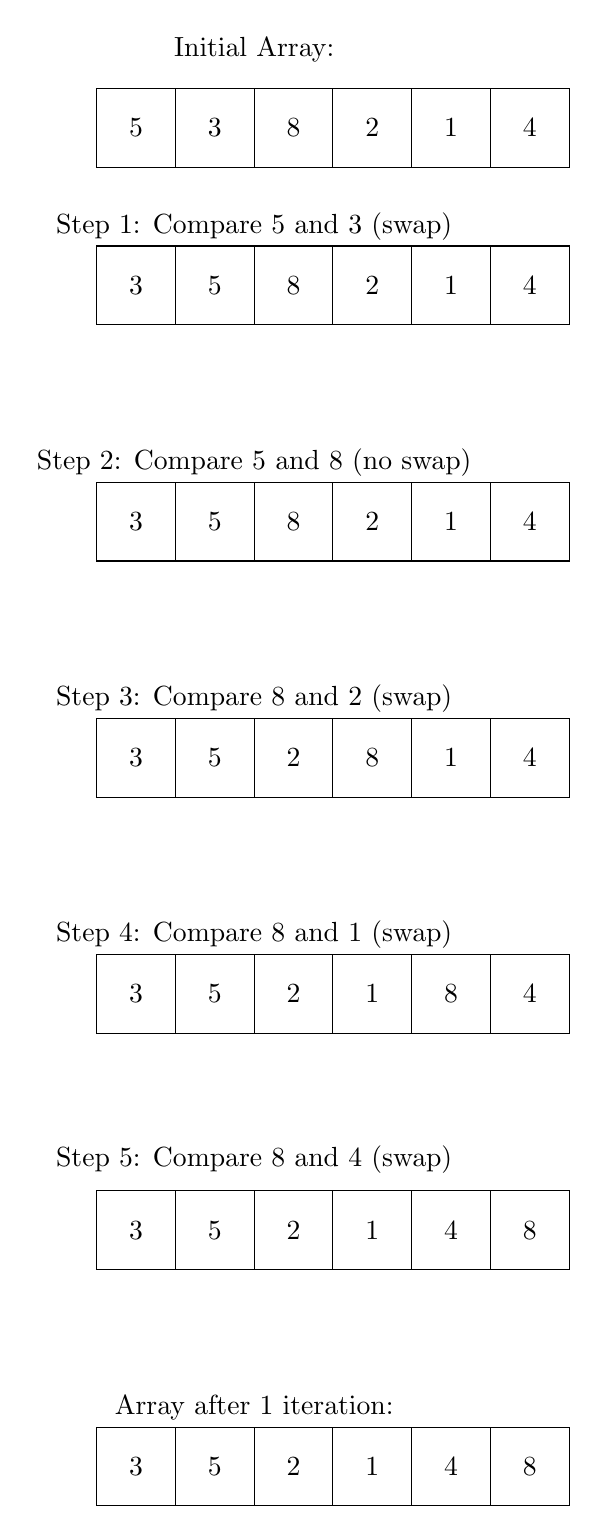
\begin{tikzpicture}

    % Initial array
    \node at (3,1.5) {Initial Array:};
    \foreach \x [count=\i] in {5, 3, 8, 2, 1, 4} {
        \draw (\i,0) rectangle ++(1,1) node[midway] {\x};
    }

    % First comparison (5 and 3)
    \node at (3,-0.75) {Step 1: Compare 5 and 3 (swap)};
    \foreach \x [count=\i] in {3, 5, 8, 2, 1, 4} {
        \draw (\i, -2) rectangle ++(1,1) node[midway] {\x};
    }

    % Second comparison (5 and 8)
    \node at (3,-3.75) {Step 2: Compare 5 and 8 (no swap)};
    \foreach \x [count=\i] in {3, 5, 8, 2, 1, 4} {
        \draw (\i, -5) rectangle ++(1,1) node[midway] {\x};
    }

    % Third comparison (8 and 2)
    \node at (3,-6.75) {Step 3: Compare 8 and 2 (swap)};
    \foreach \x [count=\i] in {3, 5, 2, 8, 1, 4} {
        \draw (\i, -8) rectangle ++(1,1) node[midway] {\x};
    }

    % Fourth comparison (8 and 1)
    \node at (3,-9.75) {Step 4: Compare 8 and 1 (swap)};
    \foreach \x [count=\i] in {3, 5, 2, 1, 8, 4} {
        \draw (\i, -11) rectangle ++(1,1) node[midway] {\x};
    }

    % Fifth comparison (8 and 4)
    \node at (3,-12.6) {Step 5: Compare 8 and 4 (swap)};
    \foreach \x [count=\i] in {3, 5, 2, 1, 4, 8} {
        \draw (\i, -14) rectangle ++(1,1) node[midway] {\x};
    }

    % Final state after one iteration
    \node at (3,-15.75) {Array after 1 iteration:};
    \foreach \x [count=\i] in {3, 5, 2, 1, 4, 8} {
        \draw (\i, -17) rectangle ++(1,1) node[midway] {\x};
    }

\end{tikzpicture}
\end{center}

You can see above that the largest integer bubbles to the top of the list.
This process illustrates a single iteration of Bubble Sort, but it is repeated until the list is sorted.

\subsection{Insertion Sort}

Insertion Sort is an algorithm that, similar to Bubble Sort, iterates through a list of elements.
It finds the smallest element in the list and places it at the beginning.
It then finds the second smallest element and places it in the second position, and so on.
The following graphic demonstrates the process of Insertion Sort:

% Tikz code for Insertion Sort
\begin{center}
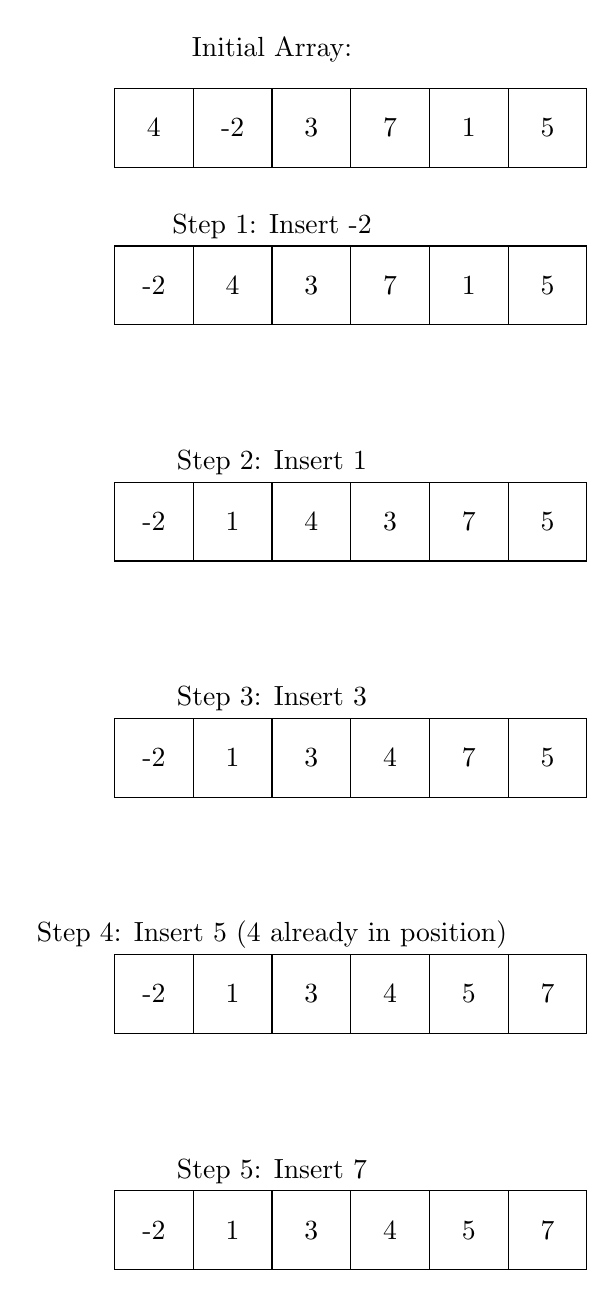
\begin{tikzpicture}

    % Initial array
    \node at (3,1.5) {Initial Array:};
    \foreach \x [count=\i] in {4, -2, 3, 7, 1, 5} {
        \draw (\i,0) rectangle ++(1,1) node[midway] {\x};
    }

    % Step 1: Insert -2
    \node at (3,-0.75) {Step 1: Insert -2};
    \foreach \x [count=\i] in {-2, 4, 3, 7, 1, 5} {
        \draw (\i, -2) rectangle ++(1,1) node[midway] {\x};
    }

    % Step 2: Insert 1
    \node at (3,-3.75) {Step 2: Insert 1};
    \foreach \x [count=\i] in {-2, 1, 4, 3, 7, 5} {
        \draw (\i, -5) rectangle ++(1,1) node[midway] {\x};
    }

    % Step 3: Insert 3
    \node at (3,-6.75) {Step 3: Insert 3};
    \foreach \x [count=\i] in {-2, 1, 3, 4, 7, 5} {
        \draw (\i, -8) rectangle ++(1,1) node[midway] {\x};
    }

    % Step 4: Insert 5
    \node at (3,-9.75) {Step 4: Insert 5 (4 already in position)};
    \foreach \x [count=\i] in {-2, 1, 3, 4, 5, 7} {
        \draw (\i, -11) rectangle ++(1,1) node[midway] {\x};
    }

    % Step 5: Insert 7
    \node at (3,-12.75) {Step 5: Insert 7};
    \foreach \x [count=\i] in {-2, 1, 3, 4, 5, 7} {
        \draw (\i, -14) rectangle ++(1,1) node[midway] {\x};
    }
\end{tikzpicture}
\end{center}

You can see above that the smallest integer is selected and placed at the beginning of the list each iteration.
This results in a sorted list at the end of the process.

\subsection{Merge Sort}

Merge Sort is a recursive algorithm that divides the list into two halves, sorts each half, and then merges the two halves together.
The first step is to recursively divide the list until the base case is reached (a list of size 1).
A list of size 1 is considered sorted.
This means that we can begin merging the lists back together in sorted order.
The following graphic demonstrates the process of Merge Sort:

% Tikz code for Merge Sort
\begin{center}
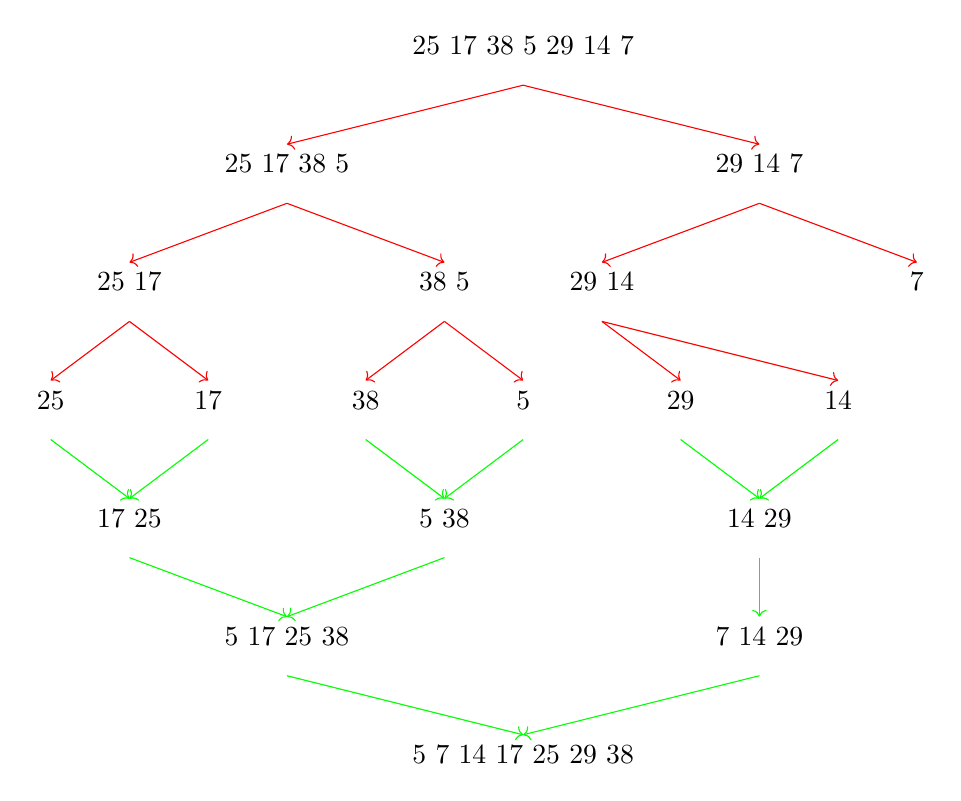
\begin{tikzpicture}
    % Nodes for the array values
    \node at (0,0) {$25\,\,17\,\,38\,\,5\,\,29\,\,14\,\,7$};
    
    % First split
    \node at (-3,-1.5) {$25\,\,17\,\,38\,\,5$};
    \node at (3,-1.5) {$29\,\,14\,\,7$};
    
    % Second split left side
    \node at (-5,-3) {$25\,\,17$};
    \node at (-1,-3) {$38\,\,5$};
    
    % Second split right side
    \node at (1,-3) {$29\,\,14$};
    \node at (5,-3) {$7$};
    
    % Third split left side
    \node at (-6,-4.5) {$25$};
    \node at (-4,-4.5) {$17$};
    
    \node at (-2,-4.5) {$38$};
    \node at (0,-4.5) {$5$};
    
    % Third split right side
    \node at (2,-4.5) {$29$};
    \node at (4,-4.5) {$14$};
    
    % Merge process (level 1)
    \node at (-5,-6) {$17\,\,25$}; % First merge left
    \node at (-1,-6) {$5\,\,38$};  % Second merge left
    \node at (3,-6) {$14\,\,29$};  % Merge right side
    
    % Merge process (level 2)
    \node at (-3,-7.5) {$5\,\,17\,\,25\,\,38$}; % Left half merge
    \node at (3,-7.5) {$7\,\,14\,\,29$}; % Right half merge
    
    % Final merge
    \node at (0,-9) {$5\,\,7\,\,14\,\,17\,\,25\,\,29\,\,38$}; % Final merge

    % Arrows indicating the flow of splitting and merging
    \draw[->, red] (0,-0.5) -- (-3,-1.25);
    \draw[->, red] (0,-0.5) -- (3,-1.25);
    
    \draw[->, red] (-3,-2) -- (-5,-2.75);
    \draw[->, red] (-3,-2) -- (-1,-2.75);
    
    \draw[->, red] (3,-2) -- (1,-2.75);
    \draw[->, red] (3,-2) -- (5,-2.75);
    
    \draw[->, red] (-5,-3.5) -- (-6,-4.25);
    \draw[->, red] (-5,-3.5) -- (-4,-4.25);
    
    \draw[->, red] (-1,-3.5) -- (-2,-4.25);
    \draw[->, red] (-1,-3.5) -- (0,-4.25);
    
    \draw[->, red] (1,-3.5) -- (2,-4.25);
    \draw[->, red] (1,-3.5) -- (4,-4.25);
    
    % Green arrows for merging
    \draw[->, green] (-6,-5) -- (-5,-5.75);
    \draw[->, green] (-4,-5) -- (-5,-5.75);
    
    \draw[->, green] (-2,-5) -- (-1,-5.75);
    \draw[->, green] (0,-5) -- (-1,-5.75);
    
    \draw[->, green] (2,-5) -- (3,-5.75);
    \draw[->, green] (4,-5) -- (3,-5.75);
    
    \draw[->, green] (-5,-6.5) -- (-3,-7.25);
    \draw[->, green] (-1,-6.5) -- (-3,-7.25);
    
    \draw[->, green] (3,-6.5) -- (3,-7.25);
    
    \draw[->, green] (-3,-8) -- (0,-8.75);
    \draw[->, green] (3,-8) -- (0,-8.75);
    
\end{tikzpicture}
\end{center}

To elaborate on the process, the list is divided into two halves until the base case is reached (a list of size 1).
When the list's are added back together, the elements are compared and merged in a sorted order.
This process is repeated until the entire list is sorted.

The following graphic represents the comparison of elements in a merge operation:

\begin{center}
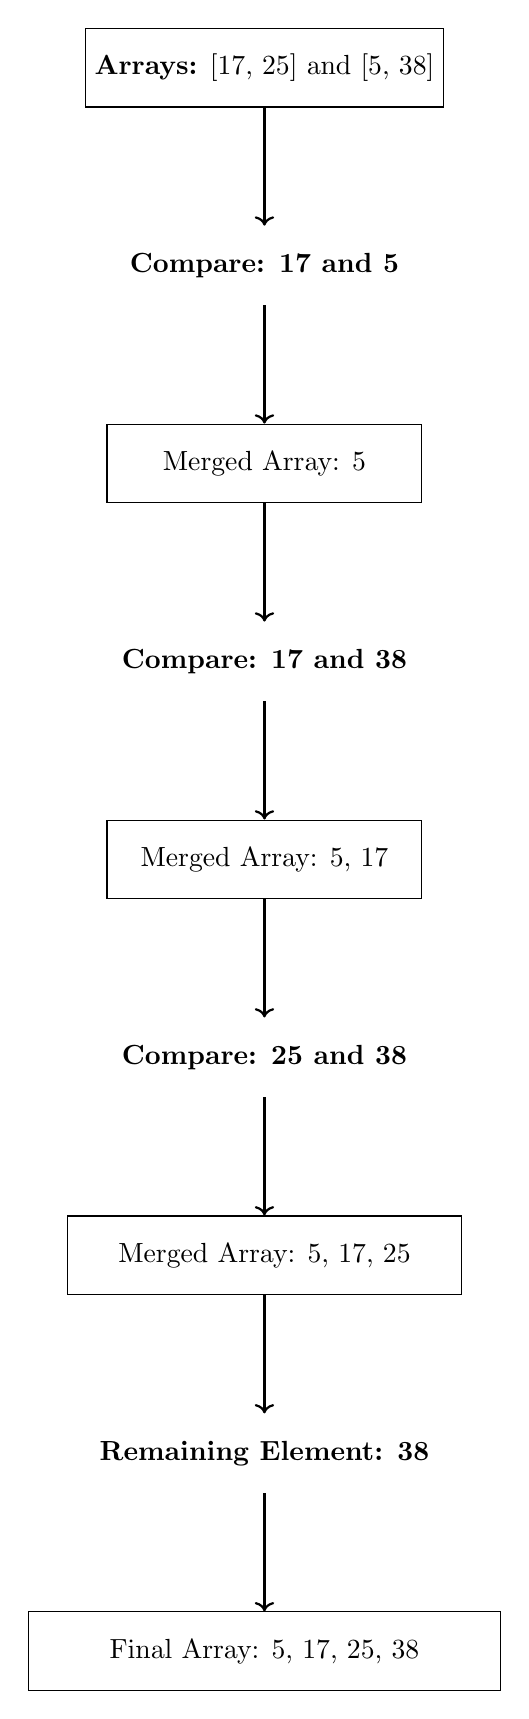
\begin{tikzpicture}[
    every node/.style={draw, rectangle, minimum width=2.5cm, minimum height=1cm, align=center},
    node distance=1.5cm
]

    % Step 1: Initial arrays
    \node (step1) {\textbf{Arrays:} [17, 25] and [5, 38]};

    % Step 2: First comparison
    \node (comp1) [below=of step1, draw=none] {\textbf{Compare: 17 and 5}};
    
    % Merged array after first comparison
    \node (merge1) [below=of comp1, minimum width=4cm] {Merged Array: 5};

    % Step 3: Second comparison
    \node (comp2) [below=of merge1, draw=none] {\textbf{Compare: 17 and 38}};
    
    % Merged array after second comparison
    \node (merge2) [below=of comp2, minimum width=4cm] {Merged Array: 5, 17};

    % Step 4: Third comparison
    \node (comp3) [below=of merge2, draw=none] {\textbf{Compare: 25 and 38}};
    
    % Merged array after third comparison
    \node (merge3) [below=of comp3, minimum width=5cm] {Merged Array: 5, 17, 25};

    % Step 5: Final element
    \node (comp4) [below=of merge3, draw=none] {\textbf{Remaining Element: 38}};
    
    % Final merged array
    \node (merge4) [below=of comp4, minimum width=6cm] {Final Array: 5, 17, 25, 38};

    % Connect arrows (straight down)
    \draw[->, thick] (step1) -- (comp1);
    \draw[->, thick] (comp1) -- (merge1);
    \draw[->, thick] (merge1) -- (comp2);
    \draw[->, thick] (comp2) -- (merge2);
    \draw[->, thick] (merge2) -- (comp3);
    \draw[->, thick] (comp3) -- (merge3);
    \draw[->, thick] (merge3) -- (comp4);
    \draw[->, thick] (comp4) -- (merge4);

\end{tikzpicture}
\end{center}

The process of merging two sorted lists involves comparing the first elements of each list and adding the smaller element to the merged list.
When this process is repeated, the merged list is sorted.

\subsection{Heap Sort}

Heap Sort consists of two main steps: building a heap and sorting the heap.
The first step involves building a heap from the list of elements.
A heap is a structure where the parent node is greater than or equal to its children.
The following graphic represents a heap structure:

\begin{center}
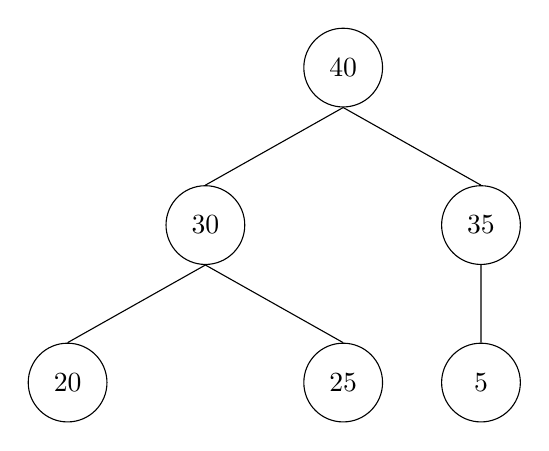
\begin{tikzpicture}[
    every node/.style={draw, circle, minimum size=1cm, inner sep=0pt},
    level distance=2.0cm,  % Increased vertical spacing
    sibling distance=3.5cm, % Increased horizontal spacing
    edge from parent path={(\tikzparentnode.south) -- (\tikzchildnode.north)}
]

    % Define nodes for a max heap
    \node {40}
        child { node {30}
            child { node {20} }
            child { node {25} }
        }
        child { node {35}
            child { node {5} }
        };

\end{tikzpicture}
\end{center}

You can see that in the heap shown above, the parent nodes are all greater than or equal to their children nodes.
When this structure is made, the root node (the largest element) is swapped with the last element in the list.
Then another heap making process is done on the remaining elements while excluding the last node (since it is already sorted).
This process is repeated until the entire list is sorted.

In array form, the heap structure is represented as follows:

\begin{center}
	\tikz \node[draw, rectangle] {40}; \hspace{0cm}
	\tikz \node[draw, rectangle] {30}; \hspace{0cm}
	\tikz \node[draw, rectangle] {35}; \hspace{0cm}
	\tikz \node[draw, rectangle] {20}; \hspace{0cm}
	\tikz \node[draw, rectangle] {25}; \hspace{0cm}
	\tikz \node[draw, rectangle] {5};
\end{center}

The left node is 2*(parent node) + 1 and the right node is 2*(parent node) + 2.

The heap making process is a recursive, bottom-up process.
It consists of comparing the parent node with its children and swapping them if the parent node is smaller.
When a swap is performed, the process is repeated on the child node that was swapped to ensure the heap property is maintained.
This process starts from the last node and works its way up to the root node.

\subsection{Counting Sort}

Counting Sort is different from the other sorting algorithms in that it requires knowledge of the range of elements in the list.
Moreover, it doesn't require comparisons between elements unlike the other sorting algorithms.
The algorithm works by counting the number of occurrences of each element in the list and then placing them in sorted order.
After knowing that fact, you can create a count array that stores the number of occurrences of each element in order of their size.

To demonstrate the process, consider the following list of elements: [4, 2, 2, 8, 3, 3, 1].
The count array would look like this: [1, 2, 2, 2, 1, 0, 0, 1].
That is, there is one 1, two 2's, two 3's, one 4, no 5's, no 6's, and one 8.
The sorted list would then be the number of occurrences of each element in order: [1, 2, 2, 3, 3, 4, 8].

While this process is simple, it requires knowledge of the range of elements in the list.
This makes it less flexible than the other sorting algorithms, but it is very efficient when the range of elements is known.

To incorporate negatives into the Counting Sort algorithm, you can add the absolute minimum value to each element in the list.
This will make all elements positive and allow the algorithm to work as intended.
In this case, the minimum value (if it's a negative) should occupy the first index in the count array, which would be 0 (negative + abs(negative) = 0).

\section{Compiling and Running the Algorithms}

To compile the sorting algorithms, you can use the following commands:

% Put it in a grey box
%gcc main.c mySort.c -o mySort
%./mySort

\begin{lstlisting}[language=bash]
gcc main.c mySort.c -o mySort
./mySort
\end{lstlisting}

The \texttt{main.c} file contains the main function that tests the different sorting algorithms.
The \texttt{mySort.c} file contains the implementation of the sorting algorithms.
When you run the compiled program, it will output the results of each sorting algorithm on a set of random integers.

To create the shared library for Python, you can use the makefile provided in the assignment.
The Makefile can be compiled by running the following command:

\begin{lstlisting}[language=bash]
make
\end{lstlisting}

The makefile as well as the \texttt{mySort.c} and \texttt{main.c} files can be found in the appendix section of this report.

\section{Space and Time Complexity}

Each algorithm was timed using the \texttt{time} module in Python.
The following table shows the time complexity of each algorithm in comparison with the built in Python \texttt{sorted} function and the \texttt{numpy.sort()} function:

\begin{center}
	\begin{tabular}{|c|c|c|c|}
	\hline
	\textbf{Algorithm} & \textbf{Time Complexity} & \textbf{Space Complexity} & \textbf{CPU Time (sec)}\\
	\hline
	Bubble Sort & $O(n^2)$ & $O(1)$ & 588.41 \\
	Insertion Sort & $O(n^2)$ & $O(1)$ & 612.63 \\
	Merge Sort & $O(n\log n)$ & $O(n)$ & 0.08 \\
	Heap Sort & $O(n\log n)$ & $O(1)$ & 0.11 \\
	Counting Sort & $O(n + k)$ & $O(k)$ & 0.02 \\
	Python \texttt{sorted} & $O(n\log n)$ & $O(n)$ & 0.40 \\
	\texttt{numpy.sort()} & $O(n\log n)$ & $O(n)$ & 0.06 \\
	\hline
	\end{tabular}
\end{center}

\subsection{Explanation of Time and Space Complexity}

\begin{itemize}
	\item \textbf{Bubble Sort:} Bubble Sort has a time complexity of $O(n^2)$ because it requires two nested loops to compare and swap elements. The space complexity is $O(1)$ because it doesn't require any additional space.
	\item \textbf{Insertion Sort:} Insertion Sort also has a time complexity of $O(n^2)$ because it requires nested loops to compare and insert elements. The space complexity is $O(1)$ because it doesn't require any additional space.
	\item \textbf{Merge Sort:} Merge Sort has a time complexity of $O(n\log n)$ because it divides the list into two halves and merges them in sorted order. We have $n$ elements and the height of the tree is $\log n$, hence the reason why this algorithm is $O(n\log n)$. The space complexity is $O(n)$ because it requires additional space to store the merged list. Since at most we'll have $n$ sublists, the space complexity is $O(n)$.
	\item \textbf{Heap Sort:} Heap Sort has a time complexity of $O(n\log n)$ because it builds a heap from the list and sorts it. The heap has $n$ elements and a height of $\log n$, hence the time complexity is $O(n\log n)$. The space complexity is $O(1)$ because it doesn't require any additional space: We can just perform operations on the original list instead of making sublists like in Merge Sort.
	\item \textbf{Counting Sort:} Counting Sort has a time complexity of $O(n + k)$ where $n$ is the number of elements and $k$ is the range of elements. This is because we need to count the occurrences of each element in the list. The space complexity is $O(k)$ because we need to store the count of each element in the list. The CPU time for Counting Sort is the lowest because it doesn't require any comparisons between elements.
	\item \textbf{Python \texttt{sorted} and \texttt{numpy.sort()}:} Both the Python \texttt{sorted} function and the \texttt{numpy.sort()} function have a time complexity of $O(n\log n)$ because they use efficient sorting algorithms. The space complexity is $O(n)$ because they require additional space to store the sorted list.
\end{itemize}

\subsection{Comparison of Algorithms}

From the table above, we can see that Merge Sort, Heap Sort, and Counting Sort are more efficient than Bubble Sort and Insertion Sort.
This makes sense because Merge Sort, Heap Sort, and Counting Sort have better time complexity than Bubble Sort and Insertion Sort.
Merge Sort and Heap Sort have a time complexity of $O(n\log n)$, which is better than the $O(n^2)$ time complexity of Bubble Sort and Insertion Sort.

In regards to the built-in Python \texttt{sorted} function and the \texttt{numpy.sort()} function, the \texttt{numpy.sort()} function is faster than the \texttt{sorted} function.
In comparison to our code, the \texttt{sorted} function is slower than our C implementations of Merge Sort, Heap Sort, and Counting Sort.
However, the \texttt{numpy.sort()} function is faster.

That being said, the Counting Sort algorithm ended up being the fastest algorithm, though it has a space complexity of $O(k)$ giving it a severe limitation.

\section{Appendix}

\subsection{mySort.c}

This file contains the implementation of the sorting algorithms in C:

\begin{lstlisting}[language=c]
// CODE: include necessary library(s)
// you have to write all the functions and algorithms from scratch,
// You will submit this file, mySort.c holds the actual implementation of sorting functions
#include "mySort.h"
#include <math.h>
#include <stdbool.h>
#include <stdlib.h>
#include <string.h>

void swap(int *x, int *y) {
    int temp = *x;
    *x = *y;
    *y = temp;
}

// Bubble Sort
void bubbleSort(int arr[], int n) {
    for (int i = 0; i < n - 1; i++) {
        for (int j = 0; j < n - i - 1; j++) {
            if (arr[j] > arr[j + 1])
                swap(&arr[j], &arr[j + 1]);
        }
    }
}

// CODE: implement the algorithms for Insertion Sort, Merge Sort, Heap Sort, Counting Sort

// Insertion Sort
void insertionSort(int arr[], int n) {

	// Iterate through each index in the array
	for (int i = 0; i < n-1; i++) { 

		// Find the lowest element in the array beyond this point and swap it with the initial point
		int *lowest = &arr[i];
		for (int j = i+1; j < n; j++) {
			if (arr[j] < *lowest) swap(&arr[j], lowest);
		}
	}
}

// Merge Sort. Given an array and the indexes of the subarray inclusive
void mergeSort(int arr[], int l, int r) {

	// Get the length of the subarray
	int n = r - l + 1;

	// Base case is when only one element is in the array
	if (n == 1) return;

	// Midpoint of the array
	int mid = (l+r) / 2;

	// Recursively split the array up
	mergeSort(arr, l, mid);
	mergeSort(arr, mid+1, r);

	// Temporary array to store the combination of the left and right arrays, both of which should be in sorted form individually
	int tmp[n];

	// Stores the indexes of the array halves
	int indexSortedL = l;
	int indexSortedR = mid+1;

	// To check if either half is empty
	bool depletedR = false;
	bool depletedL = false;

	// Iterate through the entire tmp array and assign the lesser value between the left and right half
	for (int i = 0; i < n; i++) {

		// If the current left element is less than the current right element, or if the right array has been used up, go ahead and insert into tmp
		if ((arr[indexSortedL] <= arr[indexSortedR] || depletedR == true) && !depletedL) {
			tmp[i] = arr[indexSortedL];
			indexSortedL++;

			// If all the elements have been used up make the corresponding boolean true
			if (indexSortedL > mid) {
				depletedL = true;
				indexSortedL=0; // To ensure no unsafe memory access
			}	
		}

		// If the current right element is less than the current left element, or if the left half has been used up, insert the right element into tmp
		else if (arr[indexSortedR] < arr[indexSortedL] || depletedL == true) {
			tmp[i] = arr[indexSortedR];
			indexSortedR++;

			// If all the right elements have been used up make the corresponding boolean true
			if (indexSortedR > r) {
				depletedR = true;
				indexSortedR=0; // To ensure no unsafe memory access
			}
		}
	}

	// Replace the elements in the original array with the sorted elements in the same range
	memcpy(&arr[l], tmp, n * sizeof(int));
}

// Function to make heap (used in the heapSort function)
void makeHeap(int arr[], int n, int currNodeIndex) {

	// Index of the largest amongst the parent and 2 child nodes
	int largest = currNodeIndex;

	// Get the indexes of the child nodes
	int leftChildIndex = currNodeIndex * 2 + 1;
	int rightChildIndex = currNodeIndex * 2 + 2;

	// Ensure that the left child index exists in the array
	if (leftChildIndex < n) {

		// If the left child index is greater than the existing largest (parent) assign it as the largest
		if (arr[leftChildIndex] > arr[largest]) largest = leftChildIndex;
	}

	// Ensure that the right child index is in the array
	if (rightChildIndex < n) {

		// If the right child index is greater than the existing largest (parent or left child) assign it as the largest
		if (arr[rightChildIndex] > arr[largest]) largest = rightChildIndex;
	}

	// If the largest is not the parent we started with, swap it and ensure the subheap that was swapped is still a heap
	if (largest != currNodeIndex) {
		swap(&arr[currNodeIndex], &arr[largest]);
		makeHeap(arr, n, largest);
	}
}

// Heap sort
void heapSort(int arr[], int n) {

	// Ensure we start with a max heap by going from the bottom to the top
	for (int i = n-1; i >= 0; i--) {
		makeHeap(arr, n, i);
	}

	// Begin actually sorting
	for (int i = n-1; i >= 1; i--) {

		// Swap the first and last indexes
		swap(&arr[0], &arr[i]);

		// Ensure max heap is made starting at the root node (it should be the largest)
		makeHeap(arr, i, 0);
	}
}

// Counting Sort
void countingSort(int arr[], int n) {

	// Find the maximum and minimum value in the array
	int max = arr[0];
	int min = arr[0];
	for (int i = 0; i < n; i++) {
		if (arr[i] > max) max = arr[i];
		if (arr[i] < min) min = arr[i];
	}

	// Length of the counting array should be the the number of negatives plus the number of positives plus another spot for 0
	int counts[abs(min) + max + 1];

	// Initialize the array as full of zeros
	for (int i = 0; i < abs(min) + max + 1; i++) {
		counts[i] = 0;
	}

	// Count the number of each element in the array
	for (int i = 0; i < n; i++) {

		// Increment the number of counts for whatever element is in the array
		// The minimum number is added to the index to take care of negative values
		counts[arr[i]+abs(min)]++;
	}

	// Go through the possible numbers
	int index = 0;
	for (int i = min; i <= max; i++) {

		// Put the number of each element in the array in the actual array
		// The index of number has the minimum number added to it which is to take care of negative elements
		for (int j = 0; j < counts[i+abs(min)]; j++) {
			arr[index] = i;
			index++;
		}
	}
}
\end{lstlisting}

\subsection{main.c}

This file contains the main function that tests the sorting algorithms:

\begin{lstlisting}[language=c]
// CODE: include necessary library(s)
#include <stdio.h>
#include <string.h>
#include "mySort.h"

// Utility functions
void printArray(int arr[], int n);


// Test the sorting algorithms
int main() {

	// Test cases. Uncomment the test case you want to test
    /*int arr[] = {64, 64, -134, -5, 0, 25, 12, 22, 11, 90, -500};*/
	/*int arr[] = {9, 4, 3, 8, 10, 2, 5};*/
	/*int arr[] = {3, 9, 2, 1, 4, 5};*/
	int arr[] = {15, 8, -465, -500, 8, 18, 18, 30, 10, 5, 20, 25, 8, 3, 2, 18, 6, -28, -40, -465};
	/*int arr[] = {1, 99, 56, 87, 322, 34, 2175, 217, 8};*/
	/*int arr[] = {-1};*/

	// Get the size of the array
	int n = sizeof(arr) / sizeof(arr[0]);

	// Copy the array to test the sorting algorithms
	int testArr[n];

	// Bubble Sort
	memcpy(testArr, arr, n * sizeof(int));
	printf("Original array: ");
    printArray(testArr, n);
    bubbleSort(testArr, n);
    printf("Bubble sorted array: ");
    printArray(testArr, n);
	printf("\n");

    // CODE: do the same test cases for Insertion Sort, Merge Sort, Heap Sort, Counting Sort
    // You will submit main.c, and your project will be marked based on main.c as well
	
    // Insertion Sort
	memcpy(testArr, arr, n * sizeof(int));
	printf("Original array: ");
	printArray(testArr, n);
	insertionSort(testArr, n);
	printf("Insertion sorted array: ");
	printArray(testArr, n);
	printf("\n");

	// Merge sort
	memcpy(testArr, arr, n * sizeof(int));
	printf("Original array: ");
	printArray(testArr, n);
	mergeSort(testArr, 0, n-1); // Given the start and end index inclusive
	printf("Merge sorted array: ");
	printArray(testArr, n);
	printf("\n");
    
	// Heap sort
	memcpy(testArr, arr, n * sizeof(int));
	printf("Original array: ");
	printArray(testArr, n);
	heapSort(testArr, n);
	printf("Heap sorted array: ");
	printArray(testArr, n);
	printf("\n");

	// Counting sort
	memcpy(testArr, arr, n * sizeof(int));
	printf("Original array: ");
	printArray(testArr, n);
	countingSort(testArr, n);
	printf("Counting sorted array: ");
	printArray(testArr, n);
	printf("\n");
	

    return 0;
}

// Helper functions
void printArray(int arr[], int n) {
    for (int i = 0; i < n; i++)
        printf("%d ", arr[i]);
    printf("\n");
}

\end{lstlisting}

\subsection{Makefile}

This Makefile compiles the sorting algorithms into a shared library for Python.
To compile the shared library, you can use the following command:

\begin{lstlisting}[language=bash]
make
\end{lstlisting}

The Makefile is as follows:

\begin{lstlisting}[language=make]
libmysort.so: mySort.c
	gcc -O3 -shared -o libmysort.so -fPIC mySort.c
\end{lstlisting}

\subsection{Python Code}

The raw Python code from the notebook (mySort\_test.ipynb) used to time the sorting algorithms is as follows:

\begin{lstlisting}[language=python]
"""mySort_test.ipynb

Automatically generated by Colab.

Original file is located at
    https://colab.research.google.com/drive/1QpWZWsyh7En4xVvJXfTrWkuDg-YcOtoK
"""

"""
If you are using Python on your OS, you don't need to mount your Google Drive.
You can mount your Google Drive to access files stored there. In Colab, run the
following code:
"""
from google.colab import drive
drive.mount('/content/drive')
"""
This will prompt you to authenticate and allow access to your Google Drive.
"""

"""
We use `time` to meausre the time taken by each function.
"""
import time

"""
You can use Python's `ctypes` library to interface with the C shared library.
This allows you to call functions from the shared library in Python.

After compiling your C source code and creating `libmysort.so` shared lib with:
`gcc -fPIC -shared -o libmysort.so mysort.c`,
We will be able to load the shared library named `libmysort.so` in Python using
`ctypes.CDLL` function.

Ensure the shared library is in the same directory as the Python script or in a
location where it can be found by the loader.
"""
import ctypes

"""
We use `numpy` library to create a manipulate multidimensional arrays.
"""
import numpy as np

"""
You can share the memory between Python and C directly using the ndpointer class
from the numpy.ctypeslib module. This avoids copying the data and instead passes
a pointer to the NumPy arrays underlying memory buffer. We will use ndpointer
to specify the data type of inputs to the functions.
"""
from numpy.ctypeslib import ndpointer

"""Path to the shared library on Google Drive. Mine is in this directory, you can
change it based on your needs. If you are using your own OS, not colab, just use
'./libmysort.so' if it is in the corrent directory.
"""
lib_path = '/content/drive/MyDrive/libmysort.so'

# Load the shared library
mySortLib = ctypes.CDLL(lib_path)

# Define input argument types without conversion using ndpointer
mySortLib.bubbleSort.argtypes = [ndpointer(ctypes.c_int, flags="C_CONTIGUOUS"), ctypes.c_int]
mySortLib.bubbleSort.restype = None

"""
CODE: do the same for insertion sort, merge sort, heap sort, and counting sort.
"""
mySortLib.insertionSort.argtypes = [ndpointer(ctypes.c_int, flags="C_CONTIGUOUS"), ctypes.c_int]
mySortLib.insertionSort.restype = None

# Merge sort takes an extra number input
mySortLib.mergeSort.argtypes = [ndpointer(ctypes.c_int, flags="C_CONTIGUOUS"), ctypes.c_int, ctypes.c_int]
mySortLib.mergeSort.restype = None

mySortLib.heapSort.argtypes = [ndpointer(ctypes.c_int, flags="C_CONTIGUOUS"), ctypes.c_int]
mySortLib.heapSort.restype = None

mySortLib.countingSort.argtypes = [ndpointer(ctypes.c_int, flags="C_CONTIGUOUS"), ctypes.c_int]
mySortLib.countingSort.restype = None

# Running a simple test
arr1 = np.array([64, -134, -5, 0, 25, 12, 22, 11, 90], dtype=np.int32)
n = len(arr1)
print("Original array:", arr1)

arr0 = np.copy(arr1)
mySortLib.bubbleSort(arr0, n)
print("Sorted array using Bubble Sort:", arr0)

arr0 = np.copy(arr1)
mySortLib.insertionSort(arr0, n)
print("Sorted array using Insertion Sort:", arr0)

arr0 = np.copy(arr1)
mySortLib.mergeSort(arr0, 0, n-1)
print("Sorted array using Merge Sort:", arr0)

arr0 = np.copy(arr1)
mySortLib.heapSort(arr0, n)
print("Sorted array using Heap Sort:", arr0)

arr0 = np.copy(arr1)
mySortLib.countingSort(arr0, n)
print("Sorted array using Counting Sort:", arr0)

# Creating a large test case
arr = np.random.choice(np.arange(-1000000, 1000000, dtype=np.int32), size=500000, replace=False)
n = len(arr)
print("Original array:", arr)

arr_copy = np.copy(arr)
start = time.time()
mySortLib.bubbleSort(arr_copy, n)
end = time.time()
print("Sorted array using Bubble Sort:", arr_copy)
print(f"Time to convert: {end - start} seconds")

"""
CODE: do the same for insertion sort, merge sort, heap sort, and counting sort.
"""
arr_copy = np.copy(arr)
start = time.time()
mySortLib.insertionSort(arr_copy, n)
end = time.time()
print("Sorted array using Insertion Sort:", arr_copy)
print(f"Time to convert: {end - start} seconds")

arr_copy = np.copy(arr)
start = time.time()
mySortLib.mergeSort(arr_copy, 0, n-1)
end = time.time()
print("Sorted array using Merge Sort:", arr_copy)
print(f"Time to convert: {end - start} seconds")

arr_copy = np.copy(arr)
start = time.time()
mySortLib.heapSort(arr_copy, n)
end = time.time()
print("Sorted array using Heap Sort:", arr_copy)
print(f"Time to convert: {end - start} seconds")

arr_copy = np.copy(arr)
start = time.time()
mySortLib.countingSort(arr_copy, n)
end = time.time()
print("Sorted array using Counting Sort:", arr_copy)
print(f"Time to convert: {end - start} seconds")

# Compare with built-in sort
start = time.time()
sorted_arr = sorted(arr)  # Python's built-in sort
end = time.time()
print("Sorted array with built-in sort:", sorted_arr)
print("Time taken by built-in sort:", end - start, "seconds")

# You can also use NumPy's np.sort(), which is highly optimized:
start = time.time()
np_sorted_arr = np.sort(arr)  # NumPy's optimized sort
end = time.time()
print("Sorted array using Numpy sort:", np_sorted_arr)
print("Time taken by NumPy sort:", end - start, "seconds")
\end{lstlisting}


\end{document}
